\chapter{Introdução}
A mortalidade infantil é um problema social que ocorre em escala global e a redução
dela faz parte das Metas do Desenvolvimento do Milênio, compromisso assumido pelos países
integrantes da Organização das Nações Unidas (ONU), do qual o Brasil é signatário.

A taxa de mortalidade infantil consiste na relação entre o óbito de crianças no primeiro ano
de vida e a quantidade de nascidos vivos do mesmo período. Para facilidade de comparação entre
os diferentes países ou regiões do globo esta taxa é normalmente expressa em número de óbitos a
cada mil nascidos vivos.

No Brasil tem sido observado um declínio nesta taxa, como pode-se observar no gráfico a seguir:

\begin{figure}
  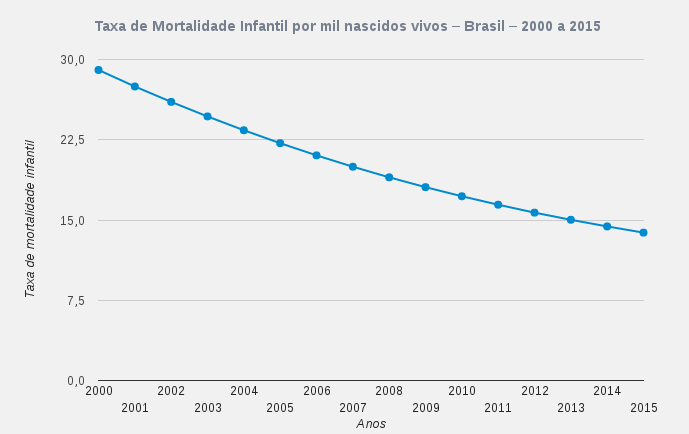
\includegraphics[width=\linewidth]{mortalidade_infantil.png}
  \caption{Gráfico}
\end{figure}
